\chapter{Desarrollo de servidor web}
\par En este capítulo se describirán los objetivos, el diseño, las prestaciones y la forma en que se llevó a cabo el montaje del servidor web.
\section{Objetivos}
\par Los objetivos de tener un servidor web que disponga de una base de datos y una interfaz visual, como lo es la pagina web son:

    \begin{itemize}
        \item Recabar la información brindada por cada lugar en donde se instale el sistema.
        \item Organizar todos los datos obtenidos en un solo lugar para que cada usuario tenga en forma remota y de fácil acceso las zonas donde se presentan este tipo de hechos. 
        \item Mostrar en forma de tabla cada una de las inhibiciones detectadas.
        \item En base a esta tabla, generar diferentes gráficos que muestren de una forma mas amigable el texto plano.
        \item Tener un lugar de soporte/sugerencias.
        \item Procesamiento matemático para la triangulación y muestra gráfica de la última detección de un lugar de interés. 
    \end{itemize}

\section{Página web}
El dominio es http://www.jammer-detector.ml y la programación de la misma fue realizada en:
\begin{itemize}
    \item HTML, el cual es usado para dar el cuerpo general de la página.
    \item CSS que nos proporciona el estilo y distribución de cada objeto.
    \item PHP, encargado de generar la conexión con la base de datos, generar el acceso de la central al servidor, entre otras funciones que se complementan a html.
    \item Javascript para generar los gráficos y el procesamiento matemático para la triangulación.
\end{itemize}
\todo[inline]{expandir conceptos de los lenguajes }

\subsection{Pestañas}
\subsubsection{Inicio}
Apenas ingresamos a la página podemos observar en la parte superior el logo y nombre del proyecto, y sobre la misma barra en la parte derecha, vemos el menú.
\par En esta pestaña de inicio se coloco la tabla donde muestra la información recabada de todos los lugares donde está instalado el sistema y se encontró una inhibición. La información que posee la misma es: ubicación, ID de cada nodo, fecha y hora y el nivel de RSSI y tipo de inhibición detectada por cada uno de los nodos. En la figura \ref{web_inicio} podemos ver la misma. 
\begin{figure}[h!]
	\centering
	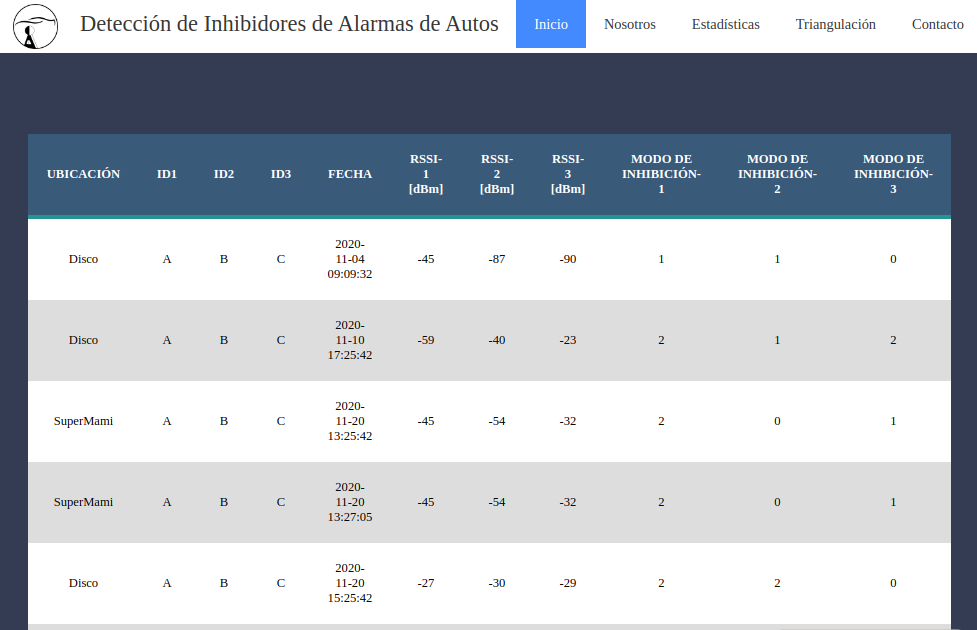
\includegraphics[scale=0.32]{images/web/tabla-web.png}
    \caption{Página de inicio}
	\label{web_inicio}
\end{figure}
\subsubsection{Nosotros}
Esta pestaña está realizada para mostrar la tarjeta de cada uno de los integrantes del grupo de trabajo, dando así también un medio de contacto.
\par En la figura \ref{web_inicio} podemos ver la pestaña. 
\begin{figure}[h!]
	\centering
	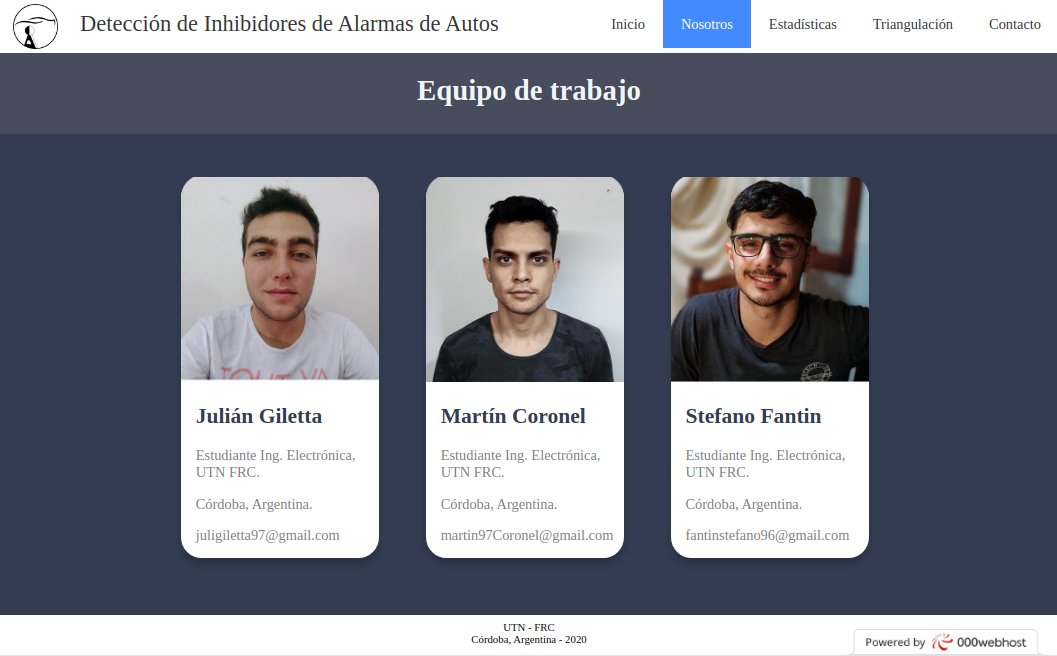
\includegraphics[scale=0.3]{images/web/nosotros-web.png}
    \caption{Presentación de grupo de trabajo}
	\label{web_nos}
\end{figure}
\subsubsection{Estadísticas}
La sección de estadísticas, quizás la mas importante para los usuarios del sistema, es en donde, de una forma gráfica y amigable, se visualizan todos los datos representados por los gráficos que mas describan la situación. 
\par En la figura \ref{web_est}, a la izquierda podemos ver un gráfico de torta con las formas de inhibiciones detectadas y a la derecha vemos un gráfico de barras que indica la cantidad de inhibiciones por cada lugar. 
\begin{figure}[h!]
	\centering
	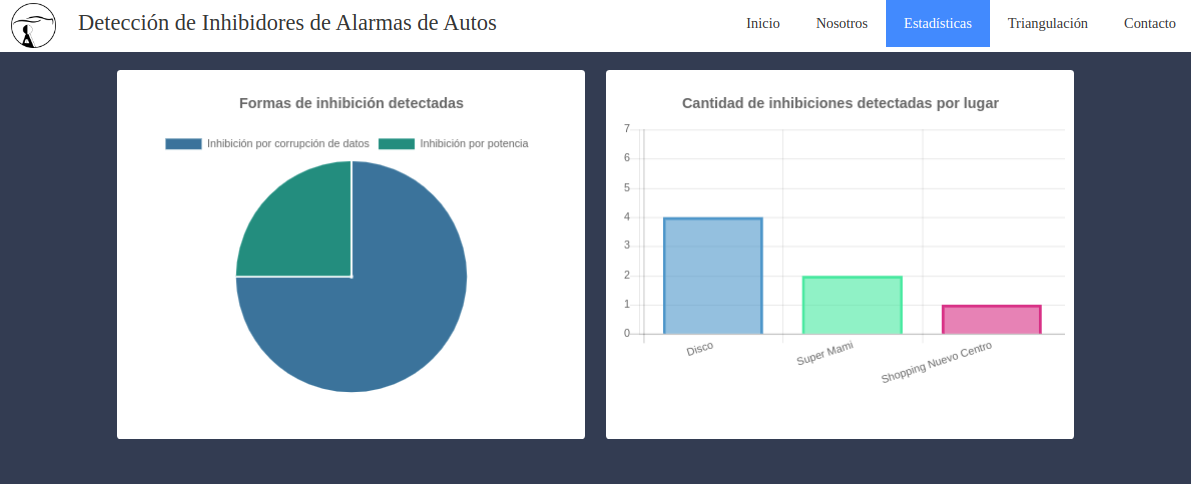
\includegraphics[scale=0.3]{images/web/est-web.png}
    \caption{Gráficos de estadísticas}
	\label{web_est}
\end{figure}
\subsubsection{Triangulación}
\par Esta sección está dedicada al procesamiento y muestra de la triángulación de inhibiciones detectadas por corrupción de
 datos con baja potencia. En la figura \ref{web_triangulacion} vemos cada vértice del triángulo que corresponde a los nodos 
 y las intersecciones de las rectas rojas que representan los límites del área donde está ocurriendo una inhibición. 
\todo[inline]{ la seccion habla de las lineas en el gráfica.. pensamos sacarlas y que haya un punto}

\begin{figure}[h!]
	\centering
	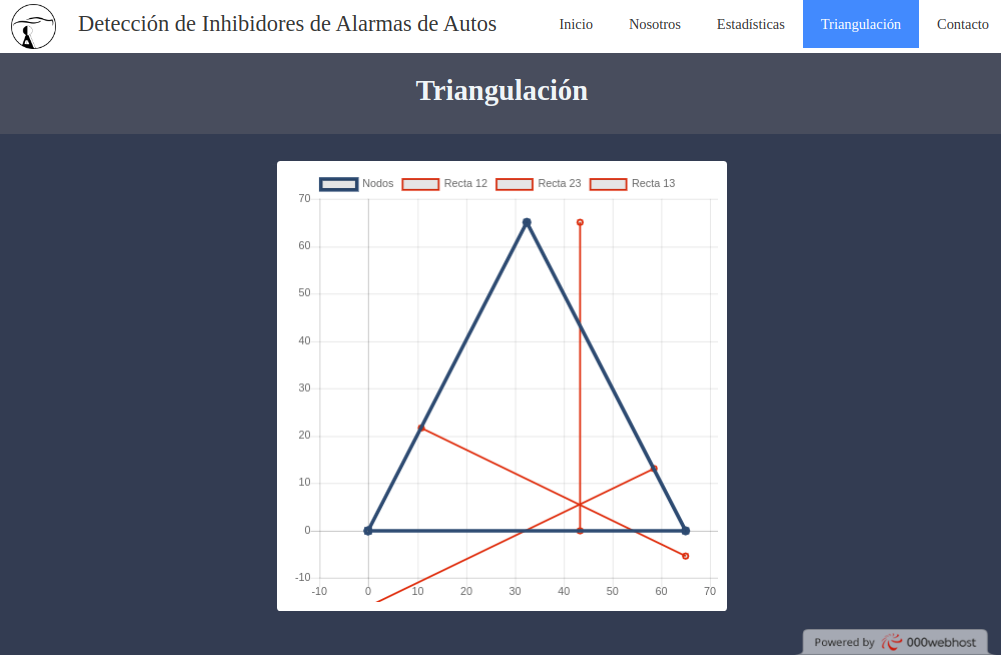
\includegraphics[scale=0.34]{images/web/triangulacion-web.png}
    \caption{Pestaña de triangulación}
	\label{web_triangulacion}
\end{figure}
\subsubsection{Contacto}
Finalmente la ultima pestaña es la de contacto, la cual tiene el fin de que cualquier persona que entre a la página y tenga alguna duda o sugerencia, pueda tener un contacto rápido con cada uno de nosotros (figura \ref{web_contacto}).
\begin{figure}[h!]
	\centering
	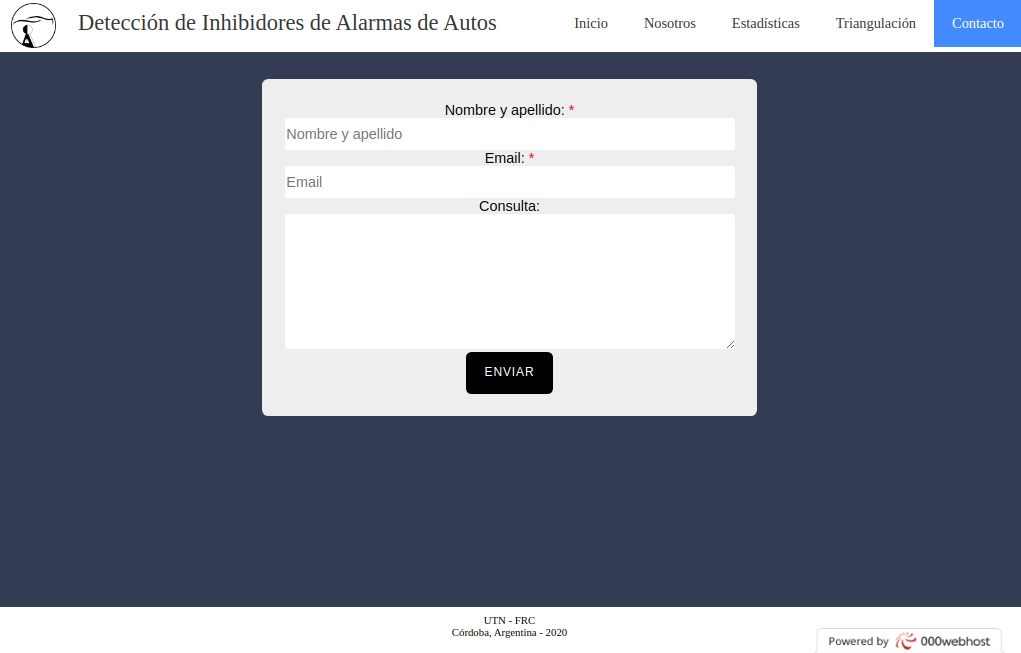
\includegraphics[scale=0.33]{images/web/contacto-web.png}
    \caption{Formulario de contacto}
	\label{web_contacto}
\end{figure}
\section{Base de datos}
La base de datos esta realizada y gestionada en phpMySQL y cuenta con una tabla con el mismo contenido que la que podemos ver en la figura \ref{web_inicio}. \par 
Es el lugar en el cual se almacena cada inhibición detectada y luego, mediante un enlace con la página web, todo su 
contenido es visualizado en esta la misma. 
\subsection{Carga de datos}
\par El enlace desde el servidor web con la central instalada en cada lugar se realiza mediante el acceso a una pestaña oculta de la web, en la cual se interactúa con la central mediante un algoritmo de http-POST-request para cargar cada uno de los datos de los nodos correspondientes a cada lugar, para luego procesarlos y obtener los gráficos ya mencionados, la triangulación en caso de ser posible y otras utilidades que se le puedan dar. 
